\section{Implementacija apstrakcije}
\label{sec:ImplementationMyAST}

Implementacija prati hijerarhije opisane u poglavlju \ref{chp:MyAST} kroz mehanizam nasleđivanja. Svaki tip čvora će biti zasebna klasa koja nasleđuje apstraktnu klasu \texttt{ASTNode}. Dijagram klasa koje nasleđuju klasu \texttt{ASTNode} se može videti na slikama \ref{fig:UMLASTNode1} i \ref{fig:UMLASTNode2}. Pored implementacije klasa koje predstavljaju AST čvorove, kreiran je i interfejs za obilazak AST-a putem obrazca posetilac.

\begin{figure}[h!]
\centering
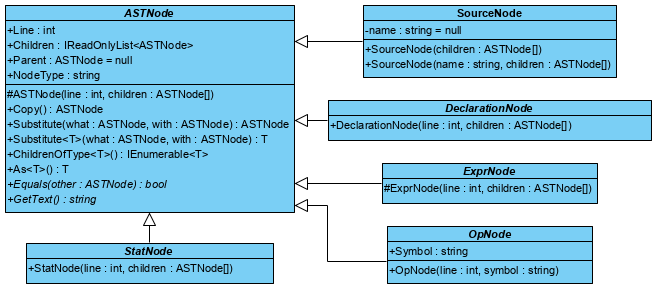
\includegraphics[scale=0.7]{images/uml/ASTNode.png}
\line(1,0){450}\\
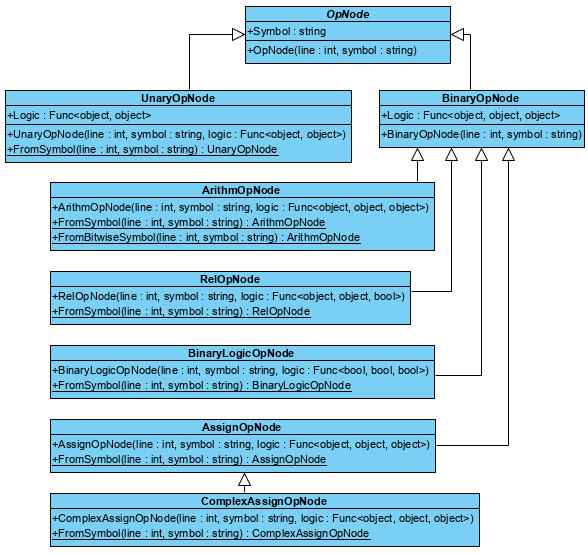
\includegraphics[scale=0.7]{images/uml/OperatorNode.png}
\caption{UML klasni dijagram (deo 1).}
\label{fig:UMLASTNode1}
\end{figure}

\begin{figure}[h!]
\centering
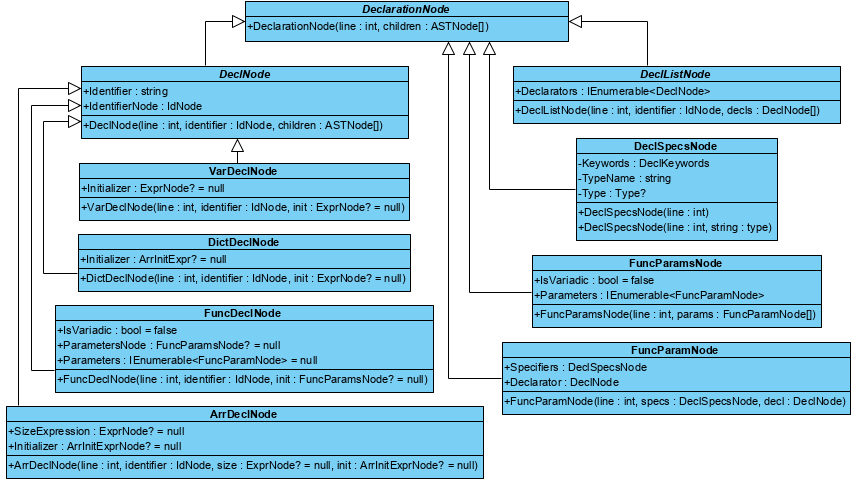
\includegraphics[scale=0.65]{images/uml/DeclarationNode.png}
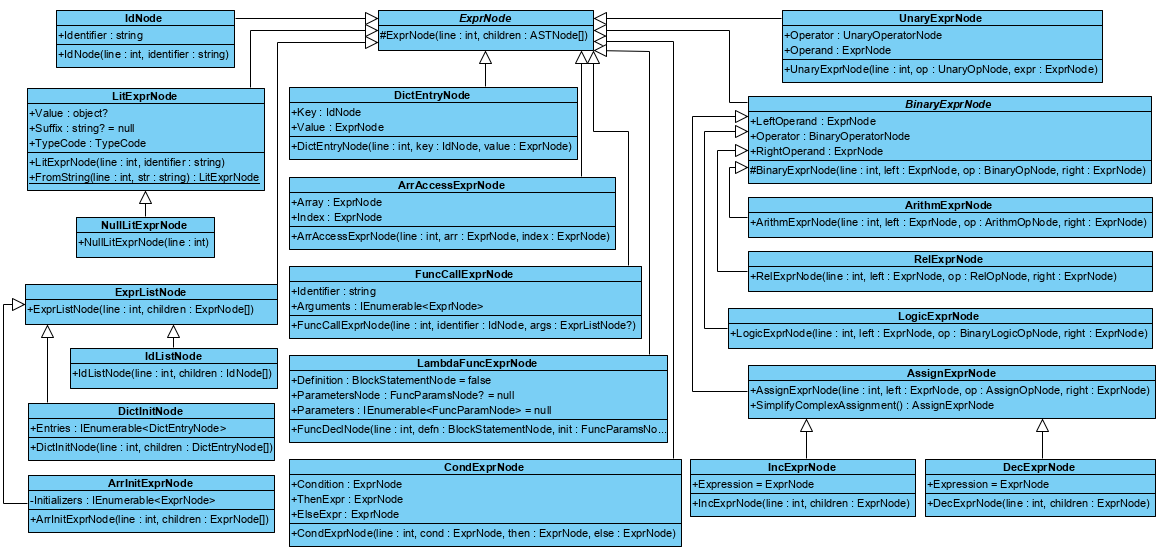
\includegraphics[scale=0.55]{images/uml/ExpressionNode.png}
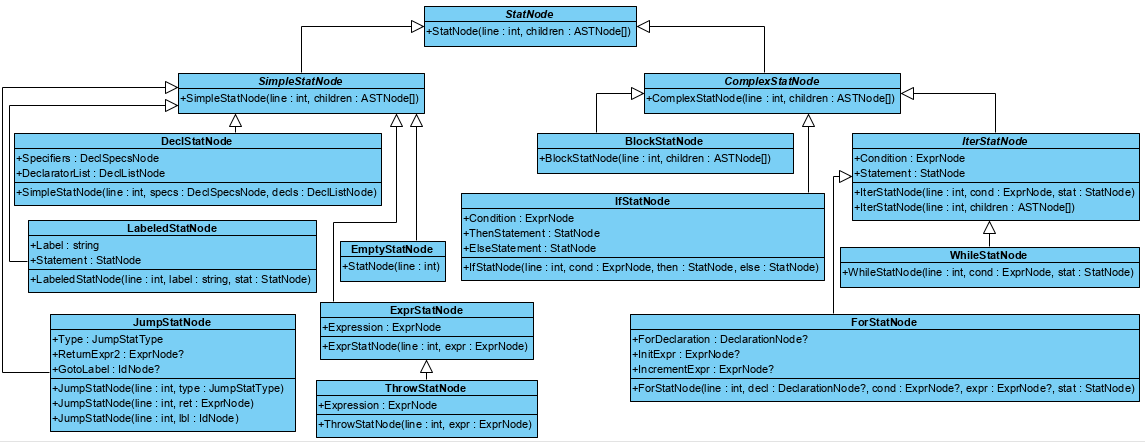
\includegraphics[scale=0.55]{images/uml/StatementNode.png}
\caption{UML klasni dijagram (deo 2).}
\label{fig:UMLASTNode2}
\end{figure}

Ovako kreirana AST struktura je \emph{imutabilna} - ne mogu se dinamički dodavati ili uklanjati deca čvorovima. Moguće je klonirati AST čvorove ili vršiti zamenu određenog podstabla drugim podstablom unutar AST-a, ne menjajući original već kopiju originala. Svaki AST čvor se može porediti po jednakosti sa drugim AST čvorom sa intuitivnom logikom poređenja pruženom kroz predefinisane operatore poređenja po jednakosti.

